% Search for all the places that say "PUT SOMETHING HERE".

\documentclass[11pt]{article}
\usepackage{amsmath,textcomp,amssymb,graphicx,enumerate,hyperref,enumitem,mathtools,tikz-qtree,listings,chemformula,bm,graphicx,grffile,gensymb,physics,amssymb,datetime,siunitx,multicol,pgfplots}
\graphicspath{{/Users/jonathansun5/Documents/Fall 2017/MCB 166/Homeworks/HW 6/Screen Shot 2017-11-29 at 11.42.43 PM.png} {/Users/jonathansun5/Documents/Fall 2017/MCB 166/Homeworks/HW 6/Screen Shot 2017-11-30 at 12.01.12 AM.png} {/Users/jonathansun5/Documents/Fall 2017/MCB 166/Homeworks/HW 6/Screen Shot 2017-11-30 at 12.08.22 AM.png} {/Users/jonathansun5/Documents/Fall 2017/MCB 166/Homeworks/HW 6/Screen Shot 2017-11-30 at 12.17.53 AM.png}}
\pgfplotsset{compat=1.14}
\makeatletter
\newcommand{\leqnos}{\tagsleft@true\let\veqno\@@leqno}
\newcommand{\reqnos}{\tagsleft@false\let\veqno\@@eqno}
\reqnos
\makeatother

\def\Name{Jonathan Sun}  % Your name
\def\SID{25020651}  % Your student ID number
\def\Homework{6} % Number of Homework
\def\Session{Fall 2017}


\title{MCB166 --- \Session --- Problem Set \Homework}
\author{\Name, SID \SID}
\markboth{MCB166 --- \Session --- Problem Set \Homework --- \Name}{MCB166 --- \Session --- Problem Set \Homework --- \Name}
\pagestyle{myheadings}
\newdate{date}{30}{11}{2017}
\date{\displaydate{date}}

\def\endproofmark{$\Box$}
\newenvironment{proof}{\par{\bf Proof:}}{\endproofmark\smallskip}

\usepackage[margin=1in]{geometry}



\begin{document}
\maketitle

\newpage
\begin{enumerate}[label=\arabic*.]
\item
The traces shown in the figure below represent synaptic currents measured under voltage clamp. The given voltages are the holding potentials with respect to the resting potential.
\begin{center}
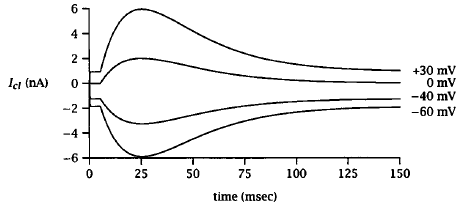
\includegraphics[width=0.75\textwidth]{/Users/jonathansun5/Documents/Fall 2017/MCB 166/Homeworks/HW 6/Screen Shot 2017-11-29 at 11.42.43 PM.png}
\end{center}
\begin{enumerate}[label=(\alph*)]
\item
What are the conductance and the reversal potential for this synaptic input?
\vspace*{1\baselineskip}
\\
ok.













\item
Is the synapse likely to be excitatory or inhibitory?
\vspace*{1\baselineskip}
\\
ok.
















\item
What is the approximate input resistance of the cell?
\vspace*{1\baselineskip}
\\
ok.
















\item
What is the approximate decay time constant of the synaptic current?
\vspace*{1\baselineskip}
\\
ok.
















\item
Is the decay time constant voltage dependent? Show the calculations that led to your answer.
\vspace*{1\baselineskip}
\\
ok.















\item
If $V_{rev}$ is not equal to $E_s$, what does this tell you about this synapse?
\vspace*{1\baselineskip}
\\
ok.














\end{enumerate}



\newpage
\item
You are voltage-clamping a neuromuscular junction at $-80 \text{mV}$ (perfect space clamp), and you measure the following end-plate currents in response to low-frequency nerve stimulation: (EPCs, in nA) $0.3$, $0.5$, $0.7$, $1.1$, $1.5$, $1.1$, $0.9$, $1.3$, $1.1$, $0.5$, $0.5$, $0.7$, $0.7$, $1.1$, $0.5$, $0.5$, $0.9$, $1.3$.
\begin{enumerate}[label=(\alph*)]
\item
If you assume that $E_s = 0 \text{mV}$, what is the approximate synaptic conductance?
\vspace*{1\baselineskip}
\\
ok.











\item
Without any knowledge about miniature EPCs, what is the mean number of quanta released per stimulus?
\vspace*{1\baselineskip}
\\
ok.











\item
From your answer in (b), what is the predicted number of failures during a $1000$-stimulus experiment?
\vspace*{1\baselineskip}
\\
ok.









\item
What are two reasons why you measure fewer failures than predicted from your calculation in (с)?
\vspace*{1\baselineskip}
\\
ok.










\end{enumerate}



\newpage
\item
You have found that two putative neurotransmitters (X and Y) cause depolarization of isolated retinal horizontal cells and that both responses reverse at $0 \text{mV}$. You want to determine whether X and Y use the same or different ligand-gated channels. You obtain the following results. In voltage clamp at $V_{\text{rest}}$, a saturating concentration of X alone causes a $2 \text{nA}$ inward current, and a saturating concentration of Y alone also causes a $2 \text{nA}$ inward current. Also, $G_{\text{rest}} = 10 \text{nS}$ and $V_{\text{rest}} = -100 \text{mV}$. Assume that there is no desensitization and that the neuron is passive (no voltage-dependent conductances).
\begin{enumerate}[label=(\alph*)]
\item
If X and Y use the same channels, calculate the expected membrane potential (under current clamp) with X alone, with Y alone, and with X and Y together. Similarly, calculate the expected total current under voltage clamp at $V_{\text{rest}}$ when X and Y are applied together.
\vspace*{1\baselineskip}
\\
ok.













\item
Repeat part (a) for the expected results if X and Y use different channels.
\vspace*{1\baselineskip}
\\
ok.













\end{enumerate}



\newpage
\item
For this problem, it is convenient to think about an equivalent circuit of the receptor cell that illustrates the action of stimulating light.
\begin{center}
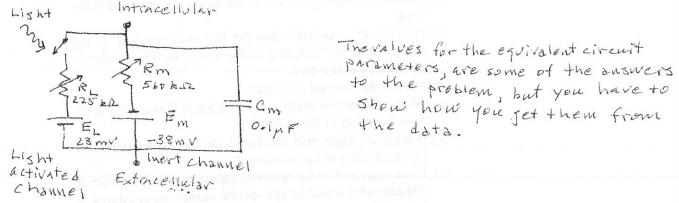
\includegraphics[width=0.75\textwidth]{/Users/jonathansun5/Documents/Fall 2017/MCB 166/Homeworks/HW 6/Screen Shot 2017-11-30 at 12.01.12 AM.png}
\end{center}
This problem concerns single visual cells in the ocellus of a barnacle (Brown, Hagiwara, Koike \& Meech, $1970$). Two glass microelectrods were inserted into the cell, one to record membrane potential and the other to pass inward or outward current pulses. At the same time a standard flash of light could be given (Fig. $13.5$).
\begin{center}
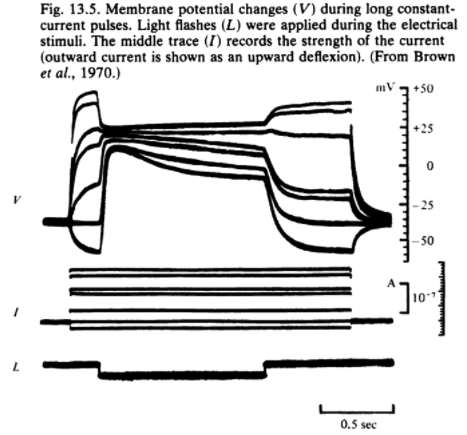
\includegraphics[width=0.75\textwidth]{/Users/jonathansun5/Documents/Fall 2017/MCB 166/Homeworks/HW 6/Screen Shot 2017-11-30 at 12.08.22 AM.png}
\end{center}
\begin{enumerate}[label=(\alph*)]
\item
Draw a text-figure graph of membrane potential against stimulus current, plotting curves for the receptor in the dark and after $0.5$ sec in the light during the flashes.
\vspace*{1\baselineskip}
\\
ok.












\item
What is the input resistance of the cell in the light and in the dark?
\vspace*{1\baselineskip}
\\
ok.












\item
Give an approximate value for the time constant  of the membrane in the dark, and deduce a value for the membrane capacitance in the dark.
\vspace*{1\baselineskip}
\\
ok.












\item
What is the reversal potential?
\vspace*{1\baselineskip}
\\
ok.











\item
What conductance change for which ion or ions is most likely to be the effect of illumination?
\vspace*{1\baselineskip}
\\
ok.












\item
Is there any clear evidence for (i) electrical excitability and (ii) rectification in the membrane?
\vspace*{1\baselineskip}
\\
ok.












\item
If you assume that the cells are spherical with a diameter of $100 \mu\text{m}$, what would be the specific membrane resistance in the dark?
\vspace*{1\baselineskip}
\\
ok.












\item
Microvilli are known to be present on the cells; how would this fact affect your estimate of specific membrane resistance?
\vspace*{1\baselineskip}
\\
ok.














\end{enumerate}



\newpage
\item
A neuron contains $N$ identical channels that are gated by the neurotransmitter glutamate. Glutamate opens these channels and results in an inward \ch{Na+} current ($E_{\ch{Na}} = +50 \text{mV}$). The glutamate-induced currents in this neuron under voltage-clamp conditions ($V_{\ch{P}} = 10 \text{mV}$) are given in the following diagram:
\begin{center}
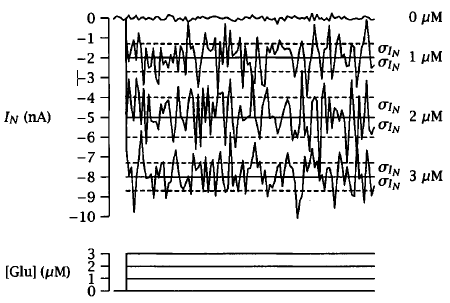
\includegraphics[width=0.75\textwidth]{/Users/jonathansun5/Documents/Fall 2017/MCB 166/Homeworks/HW 6/Screen Shot 2017-11-30 at 12.17.53 AM.png}
\end{center}
\begin{enumerate}[label=(\alph*)]
\item
Plot the variance (${{\sigma_{I}}_{N}}^2$) as a function of mean current $\mu_{I}$ on graph paper.
\vspace*{1\baselineskip}
\\
ok.












\item
Estimate the single-channel conductance and the total number of glutamate-gated channels in the neuron.
\vspace*{1\baselineskip}
\\
ok.











\end{enumerate}
\end{enumerate}
\end{document}
